\section{Representations of data}
\subsection{Outliers}
There are two common definitions of outliers. Either they are 1.5 times the inter quartile range above the upper or below the lower quartiles, or $\pm2$ standard deviations away from the mean. Often these outliers are still feasible and so left in, but sometimes an outlier doesn't make sense and should be removed from the data. An example might be an age of 200 years. This kind of outlier is called an anomaly, and the process of removing anomalies from a data set is called cleaning.

\subsection{Graphs}
\subsubsection{Box plots}
\begin{figure}[ht]
    \centering
    \incfig{an-example-box-plot}
    \caption{An example box plot}
    \label{fig:an-example-box-plot}
\end{figure}
Box plots show the quartiles as the edges of a rectangle, with the median as a line inside the rectangle. Outliers are shown with crosses, while the two whisker lines are for the lowest/highest data points that aren't outliers, or the boundaries of where outliers would be.

Comparing box plots usually involves looking at the means, ranges, or interquartile ranges and pointing out what is the same and what is different.

\subsubsection{Cumulative frequency graphs}
Cumulative frequency graphs are useful in estimating median, quartiles, and percentiles for grouped data where the exact data points are unknown. To plot a cumulative frequency diagram, an cumulative frequency table must first be drawn:
\begin{table}[ht]
\begin{tabular}{|l|l|l}
Data, $d$       & Frequency & Cumulative frequency \\
$0 \le d < 5$   & 2         & 2                    \\
$5 \le d < 10$  & 4         & 6                    \\
$10 \le d < 15$ & 6         & 12                   \\
$15 \le d < 20$ & 3         & 15                   \\
$20 \le d < 25$ & 7         & 22                  
\end{tabular}
\end{table}

\begin{figure}[ht]
	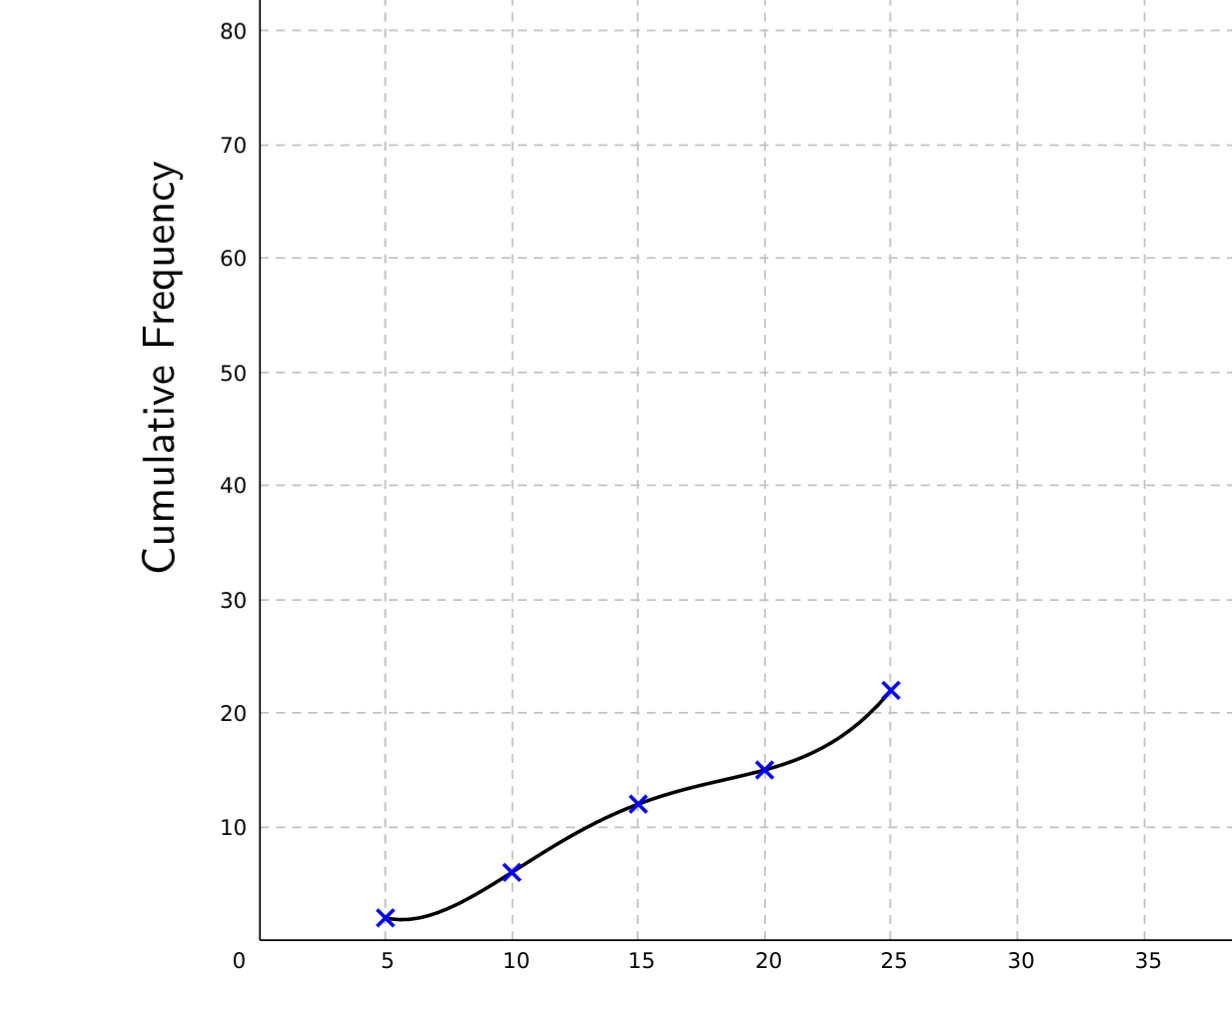
\includegraphics[scale=1.0]{cumulative-frequency-graph}
	\centering
	\caption{Example cumulative frequency graph. Note the curve should extend to 0}
\end{figure}

Estimating percentiles can be done by working out what the relevant percentile data point would be, for example the median would here be the 11th data point, and then seeing where curve is on the $y$-axis for 11 on the $x$-axis.

\subsubsection{Histograms}
Histograms are useful because they can be used on grouped data with unequal class widths. They are plotted similarly to bar charts (although with bars touching) with the data on the $x$-axis and frequency density on the $y$-axis. Frequency density is equal to frequency divided by class width, and this means that the area of a bar is equal to the frequency of the interval. By working out the area between any two points on the $x$-axis, it is possible to estimate the amount of data points between those two values.

\subsubsection{Comparing data}
Comparing data involves commenting either on measures of location, or on measures of spread. Sometimes, data will contain extreme values, which makes certain comparisions (like the median and interquartile range), better than others (for example the mean and range respectively).
